\subsection{Data Processing Pipeline}
We adopt the motion capture dataset of Van Criekinge et al.~\cite{vancriekinge2023dataset} (ages 21--86) and convert clinical marker recordings into HumanML3D-format skeletal graphs~\cite{guo2022generating} via SMPL body-model fitting~\cite{mahmood2019amass} and feature extraction, as summarized in Fig.~\ref{fig:framework} (top).
As shown in Fig.~\ref{fig:artifact}, naive mapping causes mesh inflation (right), while standard priors induce crouch artifacts (left); our multi-stage optimization pipeline adapted from VPoser~\cite{pavlakos2019expressivebodycapture3d} addresses both to recover a natural posture (center) and resolves common clinical-dataset defects such as axis misalignment, marker mislabeling, and foot contact issues.

\begin{figure}[H]
	\centering
	\IfFileExists{sec/figs/BodyArtifacts.png}%
	{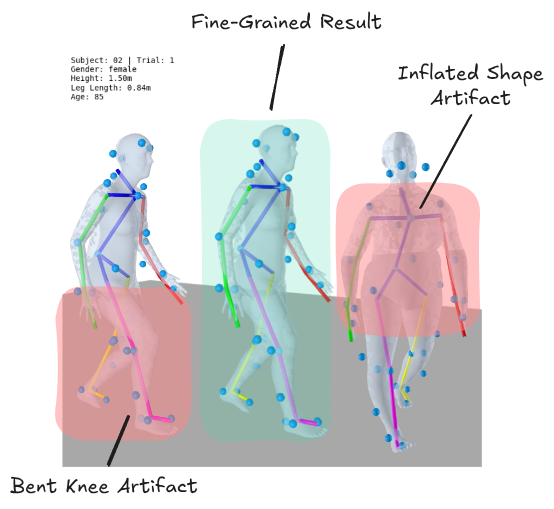
\includegraphics[width=0.7\linewidth]{sec/figs/BodyArtifacts.png}}%
	{\fbox{\parbox[c][4cm][c]{\linewidth}{\centering Artifact image missing: \texttt{sec/figs/BodyArtifacts.png}}}}
	\caption{Artifact analysis in clinical motion retargeting.}
	\label{fig:artifact}
\end{figure}

\subsection{Age Signature Detecting Network}
As illustrated in Fig.~\ref{fig:framework} (bottom left), an Age Representation Learner built on an ST-GCN~\cite{yan2018stgcn} is fine-tuned to classify motion clips into three age groups (Young, Mid, Elderly) and regress biological age.
Once the network can successfully predict age, the penultimate layer encapsulates the biomechanical signatures of aging (e.g., joint motion range).
We extract this vector to serve as the age latent embedding, denoted as $\mathbf{z}_{age}$.

\subsection{Age-Conditioned Generative Network}
Our target framework, shown in Fig.~\ref{fig:framework} (bottom right), is a Conditional Diffusion Model~\cite{tevet2023human, chen2022mld} that denoises a latent motion representation $\mathbf{x}_T$ conditioned on both text and age.
At training time, $\mathbf{z}_\text{age}$ extracted by the frozen ST-GCN encoder is injected via cross-attention, while a small MLP $g(a)$ is jointly trained to map a scalar age to the same latent space, enabling continuous age-controlled generation at inference from a desired age value alone.

Training this full architecture from scratch is infeasible under our compute and dataset budget, so the experiments in this paper validate a discrete-token prototype instead: we apply Low-Rank Adaptation (LoRA)~\cite{hu2022lora} to a pre-trained MDM with three style tokens (\texttt{young}, \texttt{mid}, \texttt{old}) and treat the continuous-conditioning architecture as the natural next step rather than a delivered contribution.
This honest scoping isolates the bottlenecks that future continuous conditioning must overcome.

\subsection{Gait-Analysis Metrics for Evaluation}
In order to validate that the aging signal is preserved in the processed dataset and successfully reproduced in the generated motion clips, we adapted several standard, training-free gait-analysis metrics documented in clinical literature~\cite{bailey2023smartwatch, cordeiro2025constraint, galasso2024development}.
\begin{itemize}
    \item \textbf{Spatiotemporal Parameters:} We compute average walking speed, stride length, and cadence by detecting heel-strike events based on the zero-velocity crossings of the ankle joints. 
    \item \textbf{Gait Variability:} We calculate the Coefficient of Variation (CV) for stride length and stride time across multiple steps. 
    \item \textbf{Joint Range of Motion (RoM):} We measure the peak flexion and extension angles of the hip and knee joints during the gait cycle. 
\end{itemize}
These metrics are computed deterministically from sample clips within our dataset and from motion generated by our LoRA-based prototype, providing a quantitative, biomechanically grounded evaluation of our framework.